\documentclass[a4paper, 12pt]{article}
\usepackage[utf8]{inputenc}
\usepackage[english]{babel}
\usepackage{apacite}
\usepackage{fancyhdr}
\usepackage{geometry}
%\usepackage{hyperref}
\usepackage[hidelinks]{hyperref}
\usepackage{amsmath, amsthm, amssymb, amsfonts}
\usepackage{marginnote}
\geometry{ left=20mm, right=20mm, top=20mm,bottom=20mm, marginparwidth=35mm}
\usepackage{graphicx}
\usepackage{caption}
\usepackage{subcaption}
\usepackage{multicol}
\usepackage{natbib}
\bibliographystyle{apacite}
\graphicspath{ {/school/printscreen/}}

\renewcommand{\vec}[1]{\mathbf{#1}}
\linespread{1}

\newcommand{\R}{\mathbb{R}}
\newcommand{\N}{\mathbb{N}}

\newcommand\fnote[1]{\captionsetup{font=small}\caption*{ #1}}

\begin{document}
\pagestyle{fancy}
\setlength{\parindent}{5ex}
\setlength{\columnseprule}{0.5pt}

\title{Summary:
\\Chapter 11 Imperfect Competition in Labor Market \\
\large Handbook of Labor Economics, Volume 4 \\
\large Alan Manning
}
\author{\url{https://github.com/s-saisw/studyGroup}}
\date{\today}
\maketitle

\rhead{Imperfect Competition in Labor Market}
\lhead{}

\begin{flushright}
Keywords: Imperfect competition; rents; search; monopsony
\end{flushright}

\begin{itemize}
\item Imperfect competition is when wage is lower than the marginal product of labor. It arises when employer, worker, or both get some rents from an existing employment relationship.
\begin{itemize}
\item Worker replacement is costly
\item An identical job cannot be found at zero cost
\end{itemize}
\item This chapter argues that model-based approach to this topic is not always helpful. Therefore, this survey only addresses general principles about imperfect competition.
\end{itemize}

\section{Sources of Imperfect Competition}
There are two types of rents: inevitable rents, and man-made rents.
\begin{enumerate}
\item Frictions and idiosyncracies: inevitable
\item Institution and collusion: man-made
\end{enumerate}
\subsection{Frictions and idiosyncracies}
\begin{itemize}
\item Frictions come from idiosyncracies in the attractiveness of different jobs rather than the lack of information.
\item Search models often assume the employer-worker match is not immediate because workers' information about the labor market is imperfect. However, this model is not very plausible since there are many employers who are recruiting and have the \emph{same characteristics} as the current employer. 
\item Frictions in labor market arise because there is a considerable idiosyncratic component to employers. e.g. non-monetary benefit, commuting distance
\item Can the internet reduce job search friction? \cite{kuhn2004internet} do not find a higher job-finding rate for those report using the internet.
\end{itemize}

\subsection{Institutions and collusion}
\begin{itemize}
\item Some institutions provide opportunities for employers to hold down wages. For example,
\begin{itemize}
\item National resident matching program (NRMP) : Hospitals collude to set medical resident wages lower than MPL.
\end{itemize}
\item Evidence is mixed whether employers collude
\begin{itemize}
\item Employers may also discuss economic conditions together and set wages accordingly.
\item Employers source of information about their rivals comes not from direct communication but from workers or business consultancies.
\end{itemize}
\end{itemize}

\section{The size of rents}
\subsection{The costs of recruitment}
\begin{itemize}
\item \emph{ Marginal hiring cos}t is used as a measure of employer rents. Let $J$ be the value of a filled job, $J_v$ the value of a vacant job, and $\theta$ the rate in which vacancies are filled. 
\begin{align*}
\text{Value of a vacant job in the next period} &+ \text{Cost of vacancy per period} \\
= &\text{Marginal hiring cost per period} \\ 
rJ_v + c=& \theta(J-J_v) 
\end{align*}

Since firms can freely create vacant jobs, $J_v=0$. Then we have
\begin{align*}
J-J_v =& \frac{c}{\theta} \\
\text{Rents} =& \text{Total cost of vacancy} 
\end{align*}
\item Denote marginal hiring cost as $h$. To see how large it is, we need to normalize by tenure and salary. Let $s$ be the separation rate, and $w$ wage. Since $1/s$ is the tenure of worker, we have
\begin{align*}
\text{How large rent is} = \frac{h}{w \cdot 1/s}=\frac{sh}{w}.
\end{align*}
\item Suppose total costs of hiring $R$ recruits are
$$
C = h_0R^{\frac{1}{\beta}},
$$
where $\beta$ is associated with return-to-scale. Then we have marginal hiring cost
$$
\frac{\partial C}{\partial R}= \frac{1}{\beta}\cdot 
{h_0 R^{\frac{1}{\beta}-1}}
=
\frac{1}{\beta} \cdot \text{average hiring cost}.
$$
If $\frac{1}{\beta}>1$, there is increasing marginal cost of recruitment.
\item Since there is not much information on hiring process, it is hard to estimate hiring costs.
\end{itemize}
\subsection{The search activity of the non-employed}
\begin{itemize}
\item The value of being unemployed can be written as
\begin{equation}
rV^u = \max_{(w^*,\gamma)}
b_u + b[1-\gamma]
+\lambda(\gamma)
\int_{w^*}
[V(w)-V^u]dF(w),
\end{equation}
where \\
$V^u$ : value of being unemplolyed \\
$\gamma$ : time spent on job search \\
$w^*$ : reservation wage. Note that it is also a choice variable.\\
$b_u$ : income received when unemployed \\
$b$ : value of leisure \\
$\lambda$ : arrival rate of job offers (function of $\gamma$) \\
$F(w)$ : wage offer distribution \\
$V(w)$ : value of job that pays $w$ \\

Taking FOC for $\gamma$, then
\begin{equation}
b = \lambda'(\gamma)
\int_{w^*}
[V(w)-V^u]dF(w),
\end{equation}
 This means time spent on job search depends on the rents workers will get from offer. 
\item Rearrange the terms and obtain
\begin{align*}
\frac{\int_{w^*}
[V(w)-V^u]dF(w)}
{1-F(w^*)}
=&
\frac{b}{1-F(w^*)}
\cdot
\frac{1}{\lambda'(\gamma)}\\
=&
\frac{b}{1-F(w^*)}
\cdot
\frac{1}{\lambda}
\cdot
\frac{\lambda}{\lambda ' (\gamma)}\\
=&
\frac{bd_u \gamma}{\epsilon_{\lambda \gamma}},
\end{align*}
where \\
$\frac{1}{d_u}=\lambda(1-F(w^*))$ : is the rate which job offers arrive $\times$ the fraction of acceptable jobs i.e. expected duration of employment \\
$\epsilon_{\lambda \gamma}$ : elasticity of job arrival rate to search time\\
This means the average rent is equal to the opportunity cost of time looking for a job divided by elasticity.

\item Then we can derive the formula for the gap between the average wage and reservation wage. (See Appendix A.)
\begin{equation}
\frac{\bar{w}-w^*}{w^*}
=
(1-\rho)
\frac{\gamma}{\epsilon_{\lambda \gamma}[1-\gamma]+\gamma}
\cdot
\frac{u}{1-u},
\end{equation}
where $\rho =  \frac{b_u}{w^*}$ and $u$ is the steady state unemployment rate for worker.

\item We want to estimate average rents (LHS) , monetary value of leisure ($b$), total time spent until getting a job ($d_u$), elasticity of job offer arrival rate ($\epsilon_{\lambda \gamma}$)


\item Evidence suggests $\gamma$ is small. 
\begin{itemize}
\item One explanation for this is workers quickly exhaust existing vacancies then search among new inflow of vacancies. Therefore, there is little return for extra job search effort.
\end{itemize}
\item Since there are inactive people, there must be some heterogeneity in the size of job rents. People with smaller rents do not look for jobs.
\end{itemize}
\subsection{The costs of job loss}
\begin{itemize}
\item To estimate workers' rents for employment, we want to consider what happens  when workers are randomly separated from jobs.
\begin{itemize}
\item This topic is studied in the literature concerning displaced workers.
\item Prior to the separation, there is little difference in wage between treatment and control groups. However, a gap between these groups arises after displacement.
\end{itemize}
\end{itemize}

\section{Models of wage determination}
\begin{itemize}
\item There are two ways wage can be determined:
\begin{enumerate}
\item Ex post wage-bargaining 
\begin{itemize}
\item Wage is determined after employer and worker have been matched (usually by asymmetric Nash bargain)
\item Preferred in macroeconomic applications
\item Bargaining power of worker is assumed to be \emph{exogenous}
\item If firm productivity is greater than worker's leisure value, there is surplus to be shared between employer and worker. Therefore the match with positive surplus is always consummated.
\end{itemize}
\item Ex ante wage-posting
\begin{itemize}
\item Wage is set unilaterally by the employer before employer and worker are matched.
\item Preferred in microeconomic applications
\item Bargaining power of worker depends on \emph{elasticity of labor supply} curve to the firm. If labor supply is less elastic, employer has more bargaining power. If wage is cut at the same amount, there are less workers who leave jobs. \\ cf. standard monopsony model
\begin{figure}[h]
\centering
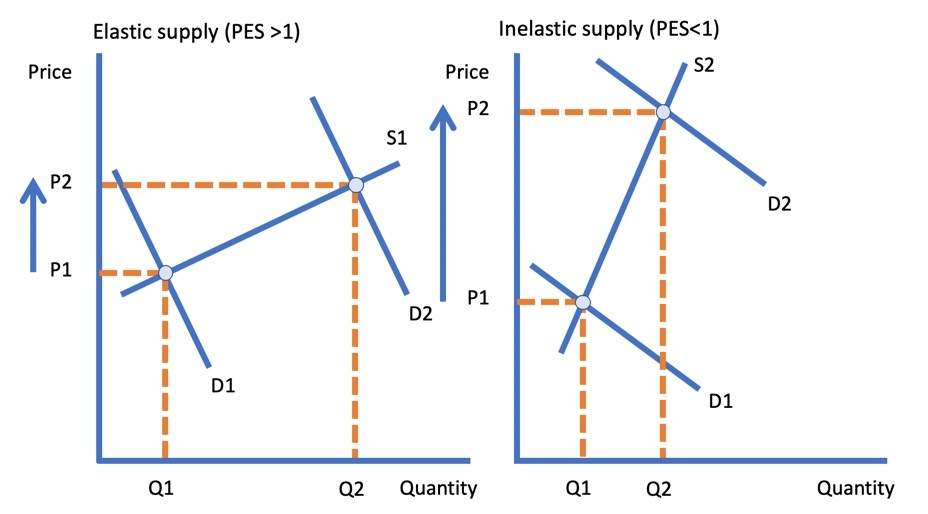
\includegraphics[scale=0.5]{supply_elasticity.jpg}
\fnote {Source: tutor2u.net}
\end{figure}
\item Match with positive surplus may not be consummated if wage is set lower than leisure value of individuals $\Rightarrow$ inefficient
\end{itemize}
\end{enumerate}
\item Consider the following static models. Suppose $p$ is firm productivity, and $b$ is leisure value of worker.
\begin{enumerate}
\item Wage-bargaining model \\
Wage is chosen to maximize an asymmetric Nash bargain:
\begin{equation}
(p-w)^{1-\alpha}(w-b)^\alpha
\end{equation}
Then, 
\begin{equation}
w = \alpha p + (1-\alpha)b.
\end{equation}
\item Wage-posting model \\
A worker will accept offer if $w>b$. Suppose $G(w) = (w-b_0)^\epsilon$ is labor supply function and $b_0$ is the lowest wage any workers accept. Firm sets wage to maximize
\begin{equation}
\pi(w) = (p-w)G(w)
\end{equation}
Then
\begin{equation}
w = 
\frac{\epsilon}{1+\epsilon}p
+
\frac{1}{1+\epsilon}b_0.
\end{equation}
\end{enumerate}
\item Theoretically, wage-bargaining model is more efficient. However, empirical evidence suggests both exist.
\begin{itemize}
\item \cite{hall2008wage} find negotiation is more common in high-skilled labor markets.
\item  Bargaining suggests there would be variation within firms between workers with different reservation wage; while posting suggests there is no variation within firm even if reservation wage is different. \cite{machin2004test} find wage variation between firms rather than within firms.
\end{itemize}
\end{itemize}
\section{Estimates of rent-splitting}
In this section we consider the estimates rent sharing parameter of worker in both wage-bargaining model and wage-posting model.
\subsection{Estimates of rent sharing}
\begin{itemize}
\item Consider wage-bargaining model. Rent sharing parameter is represented by bargaining power of workers.
\item Consider the following Nash bargaining model. Wages and employment $N$ are chosen to maximize
\begin{equation}
[F(N)-wN]^{1-\alpha}
[N(w-b)]^\alpha,
\end{equation}
where \\
$F(N)$ : revenue function \\
$b$ : leisure value \\
Then FOC wrt wage can be written as
\begin{equation}
w = \alpha \frac{F(N)}{N}+(1-\alpha)b.
\label{eq:wagebargain}
\end{equation}
That is, wage is a weighted average of revenue per worker and worker's leisure value.\footnote{Similarly, FOC wrt employment is
$$
N(1-\alpha)(F'(N)-w)+\alpha[F(N)-wN]=0.
$$
Then we can solve for employment level. Employment must satisfy
\begin{equation}
F'(N) = b
\end{equation}
}
\item We may estimate \eqref{eq:wagebargain} with data. Variation of estimating equation includes
\begin{align}
w =& \frac{\alpha}{1-\alpha}
\frac{F(N)-wN}{N}+b \\
=&
\frac{\alpha}{1-\alpha}
\frac{\Pi}{N}
+b
\end{align}
We can obtain data on profit per worker and wage. $b$ is unobserved. However, OLS estimation of \eqref{eq:wagebargain} is biased since $\frac{\Pi}{N}$ is potentially endogenous to wages. 
\item To fix this problem, we may consider instrument that affects revenue function but does not affect wage. However, instruments based on revenue shifters are often weak.
\begin{proof}
Suppose the revenue function is Cobb-Douglas, i.e. $F(N) = N^k$. Then
$$
F'(N) = k\frac{F(N)}{N}=b.
$$
Let instrument $z$ satisfies exclusion restriction. Then it is not correlated with $b$. However, since $F(N)=kbN$ and $k$ is constant, $z$ is also weakly correlated with $F(N)$. Thus, $z$ is weak instrument.
\end{proof}
\item Many studies use profit data at firm level but demand shifter at industry level. However, industry level demand shifter may also be endogenous. It is possible positive shock to the industry raises labor demand, and general level of wage ($b$) is increased consequently. Therefore, estimates are biased upwards.
\item Emprirical studies often focus on unionized firms. But studies that compare union and non-union sectors often find $\alpha$ is larger in non-unionized firms. This is consistent with the wage-posting model. It is possible that in wage-posting model, non-unionized firms face a more elastic labor supply.
\end{itemize}

\subsection{Elasticity of labor supply curve to an individual employer}
\begin{itemize}
\item Consider wage-posting model. To estimate the size of rent sharing, we need to estimate the elasticity of labor supply first.
\item Ideally, we want to estimate the labor supply elasticity of each firm. We can randomly vary the wage and observe how labor supply changes.
\item Empirical studies have used quasi-experiment to estimate the labor supply elasticity. The following studies consider the change in employment following mandatory \emph{wage increase} in the short run.
\begin{itemize}
\item \cite{staiger2010there} find the elasticity in labor supply of nurses is \textit{low} (0.1). This suggests $\alpha$ is low. $\Rightarrow$ Hospitals have monopsony power.
\item \cite{falch2010elasticity} also find small elasticity (1.0--1.9) for teachers.
\end{itemize}
\item Another way to think about labor supply elasticity is to consider it as an inverse of wage elasticity, i.e. we can look at the impact of \emph{employment increase} on wage.
\begin{itemize}
\item \cite{matsudaira2014government} investigate the impact of mandated increase in the level of employment on wage. Firms do not raise wage. $\Rightarrow$ wage elasticity is low. $\Rightarrow$ Labor supply elasticity is \emph{high}.
\end{itemize}
\item Conflicting evidence can be explained by
\begin{itemize}
\item ``Generalized model of monopsony'' \citep{manning2006generalised}. Firms have to pay hiring cost. Firms can adjust recruitment activity instead of changing wage or employment level.
\begin{itemize}
\item When mandated wage increases, labor supply to firm increases. However, firm can adjust by reducing recruitment activity, leaving employment level unchanged.
\item When mandated employment increases, firm recruits more workers to make the wage unchanged.
\end{itemize}

\item Heterogeneous workforce
\begin{itemize}
\item When mandated wage increases, firm hires only high-quality worker. $\Rightarrow$ Employment level is unchanged.
\item When mandated employment increases, firm hires a lot of low-quality workers. $\Rightarrow$ Wage remains unchanged.
\end{itemize}
\end{itemize}
\item These studies have not considered the impact of wage on labor supply an \emph{individual} firm faces.
\end{itemize}

\subsection{The sensitivity of separation to wages}
\begin{itemize}
\item Elasticity of separation with respect to wage can also be used to compute the elasticity of labor supply.
\begin{proof}
At steady state
\begin{align*}
\text{Recruit} =& \text{Separation} \\
R(w) =& s(w)N(w),
\end{align*}
where \\
 $r(w)$ : flow of recruits to a firm \\
 $s(w)$ : separation rate \\
 Take derivative with respect to wage. Then,
 \begin{align*}
\frac{\partial R}{\partial w}
=&
\frac{\partial N}{\partial w} \cdot s
+
\frac{\partial s}{\partial w} \cdot N \\
\epsilon_R \cdot \frac{R}{w} 
=&
\epsilon_N \cdot \frac{sN}{w}
+
\epsilon_s \cdot \frac{sN}{w} \\
\epsilon_N =& \epsilon_R - \epsilon_s
 \end{align*}
 
In fact, both elasticity of recruits and elasticity of separation are both important to estimate the elasticity of labor supply facing a firm.
\end{proof}

\item Quasi-experiment studies report separation elasticity ranging from 0.25--4.
\begin{itemize}
\item These differences may have come from the fact that they consider different labor markets.
\item The lack of control group is also a problem in these studies. They study the change in minimum wage and living wage which affects the whole market. Ideally, we would want to consider change in wage of a single firm, holding wages of other firms constant.
\end{itemize}
\item Non-experimental studies report separation elasticity ranging from 0.25--1.9. They differ in many dimensions, such as
\begin{itemize}
\item Definition of separation: quit rate VS involuntary lay-offs 
\begin{itemize}
\item Involuntary lay-offs are more sensitive to wage increases than quits.
\end{itemize}
\item Definition of wage: current wage VS future prospects of wage
\begin{itemize}
\item Permanent component of wage is more likely to affect separation than current wage.
\end{itemize}
\item Controlling for average level of wages in labor market
\begin{itemize}
\item Average wage in the labor market can be thought of individual permanent wage component that is not specific to any firm.
\item Average wage is positively correlated with wage but negatively correlated with separation (Individual with high human capital quit less).
\item Failing to control for average wage upward biases the estimates.
\end{itemize}
\item Controlling for job tenure
\begin{itemize}
\item Tenure is positively correlated with wage but negatively correlated with separation. Tenure here serves as a proxy for ability. Failing to control for tenure will violate exogeneity assumption. 
\item However, if there are seniority wage scales, tenure grows with wage. When regress wage on separation and simultaneously control for tenure, tenure itself becomes outcome variable, indicating bad control.
\end{itemize}
\end{itemize}
\item In addition to separation elasticity, we also need recruitment elasticity. Studies equate recruitment elasticity to the separation elasticity since \emph{average} quit elasticity and recruit elasticity must be the same across economy, although those of individual firm may not be (Proof is provided in section 4.3.3).
\item Consider the following monopsony model with hiring cost. Consider a monopsonistic employer who chooses wage and recruitment intensity to maximizes steady state profits:
$$
\Pi = F(N) -wN-H.
$$
Suppose number of recruit depends on wage and hiring cost. Then we can derive 
\begin{equation}
N(w,H) =
\frac{R(w,H)}{s(w)}
=
\left(
\frac{H}{\tilde{H}}
\right)^{\beta}
\frac{R(w)}{s(w)}
=
\left(
\frac{H}{\tilde{H}}
\right)^{\beta}
n(w),
\label{eq:laborsupply}
\end{equation}
where \\
$\tilde{H}$ : aggregated hiring activity of the economy \\
$\beta$ : parameter that represents the shape of hiring cost curve. If $\beta<1$, marginal hiring cost curve is increasing in the number of recruit. 
\begin{itemize}
\item Since $N$ is a function of wage, we obtain FOC for wage as follows
\begin{equation}
\frac{\partial \Pi}{\partial w} = 0
\Rightarrow
w = \frac{\epsilon}{1+\epsilon}F'(N),
\end{equation}
where $\epsilon$ is the elasticity of labor supply with respect to wage. This means there is a gap between MPL and wage. If $\epsilon$ is low (labor supply increase is small compared to the increase in wage), the gap is large.
\item Next, we obtain FOC for recruitment intensity. Since $N$ is a function of $H$, 
\begin{equation}
\frac{\partial \Pi}{\partial H} = 0
\Rightarrow
\frac{H}{N}
=
\beta [F'(N)-w].
\end{equation}
\item Combining the two FOCs, we obtain
\begin{equation}
\frac{H}{wN}=\frac{\beta}{\epsilon}
\end{equation}
We can use this equation to calculate $\beta$ from data. Empirical evidence suggests $\beta<1.$ 
\end{itemize}
\end{itemize}
\subsection{Measuring labor market frictions}
\begin{itemize}
\item Another approach to measure the degree of rent splitting is the degree of competition among employers. One particular measure in the literature is the ratio of arrival rate of job offers for an employed workers to the rate employees leave employment to unemployment, $k$.
$$
k=
\frac{\lambda_e}{\delta}
$$
The higher the $k$, the higher competition among employers and higher wage.
\item $k$ can be used as alternative measure for balance of power between workers and employers. However, if workers have other motivation that wage or future wage when change jobs, $k$ may not be a good measure.
\item Compared to the measure based on wage elasticity of supply curve, $k$ is relatively easy to compute. However, since it is based only on the data on labor market transition, many assumptions may not hold.
\end{itemize}
\section{Applications}
\subsection{(The failure of) the law of one wage}
\begin{itemize}
\item Imperfect competition can explain why there is wage dispersion in the labor market.
\begin{itemize}
\item In perfectly competitive market, labor supply is perfectly elastic.
\item Therefore, all employers pay the same wage.
\end{itemize}
\item In wage-bargaining model, wage dispersion comes from the difference in productivity and reservation wage.
\begin{itemize}
\item This scenario cannot happen in perfectly competitive market as it assumes homogenous products (workers).
\end{itemize}
\item In wage-posting model, \cite{burdett1998wage} present a model that explains wage dispersion among homogeneous workers and employers. The equilibrium is a wage distribution with no mass point.
\begin{itemize}
\item However, the result is based on the assumption that all workers move for the smallest gain in wages.
\item Mass point in wage distribution is observed in real world, e.g. around minimum wage. 
\end{itemize}
\end{itemize}
\subsection{Labor market regulation}
\begin{itemize}
\item Labor market regulation is only justified when market is not perfectly competitive.
\item The simple model of monopsony suggests that artfully chosen minimum wage raises employment. However, a more complicated model of monopsony suggests this may not be the case. General monopsony model predicts a smaller employment increase than simple monopsony model.
\begin{proof}  
Consider the monopsony model with hiring cost. In addition, assume $F'(N)=p$ for simplicity. For any wage, the FOC with respect to hiring cost is
\begin{align*}
\frac{\partial \Pi}{\partial H} = 0
\Rightarrow
p-w =& \frac{1}{\beta N}
\left[
\frac{N}{n(w)}
\right]
^
{
\frac{1}{\beta}
} \\
N =&
n(w)^\frac{1}{1-\beta}
[
\beta
(p-w)
]^
\frac{\beta}{1-\beta}.
\end{align*}
Then, the optimal employment level is given by
\begin{equation}
\frac{\partial N}{\partial w} = 0
\Rightarrow
w^* = \frac{\epsilon}{\beta+\epsilon}p
\end{equation}
Next, consider the simple monopsony model. Recall employer chooses
\begin{equation}
w^m = \frac{\epsilon}{1+\epsilon}p
\end{equation}
Since empirically $\beta<1$, we have $w^*>w^m$. Thus, when minimum wage increases, since $w^*$ is originally higher, employment gain is less.
\end{proof}
\item This model, however, still ignores some important reality.
\begin{enumerate}
\item By using a model with single monopsonist, it automatically assumes every employer faces the same labor supply curve
\item It also ignores that employers may choose different wage prior to minimum wage increase.
\end{enumerate}
\cite{manning2003monopsony} shows that by incorporating the above two assumptions, minimum wage \textit{always} reduces employment.
\end{itemize}
\subsection{The gender pay gap}
\begin{itemize}
\item If labor supply of women is less elastic than men, employers may choose to pay smaller wage for women e.g. More women may stop working if wage is reduced but men will stay.
\item Recent studies have focused on checking if the separation elasticity\footnote{As noted in section 4.3, lower separation elasticity means lower elasticity of labor supply.} of women is lower than men.
\item  Empirical studies find this is true. However, estimates are sensitive to specifications.
\end{itemize}
\subsection{Economic geography}
\begin{itemize}
\item Monopsony power can help explain why large employer locates in the city and smaller employer locates in rural areas.
\item Firms can only have power over workers if they are isolated. However, there are also fewer workers.
\item In the rural area, there are fewer workers. Only firms who want low level of employment choose rural area and exercise the monopsony power.
\item It is more beneficial for firms who want to  have a higher level of employment or more volatile employment to locate in urban area.
\end{itemize}
\subsection{Human capital accumulation and training}
\begin{itemize}
\item Imperfect competition can explain why firms pay training costs.
\begin{itemize}
\item In perfect competition, workers obtain all the returns to human capital.
\item \cite{acemoglu1997training} finds wage is lower than MPL.
\end{itemize}
\item In imperfect competition, employers pay for training in order to increase future supply of labor. \\
cf. \cite{benson2013firm} Hospital sponsor students to train as nurses.
\end{itemize}
\bibliographystyle{apacite}
\bibliography{imperfectCompetition} 


\end{document}
